\documentclass{standalone}
\usepackage{tikz}
\usetikzlibrary{patterns, positioning}


\begin{document}
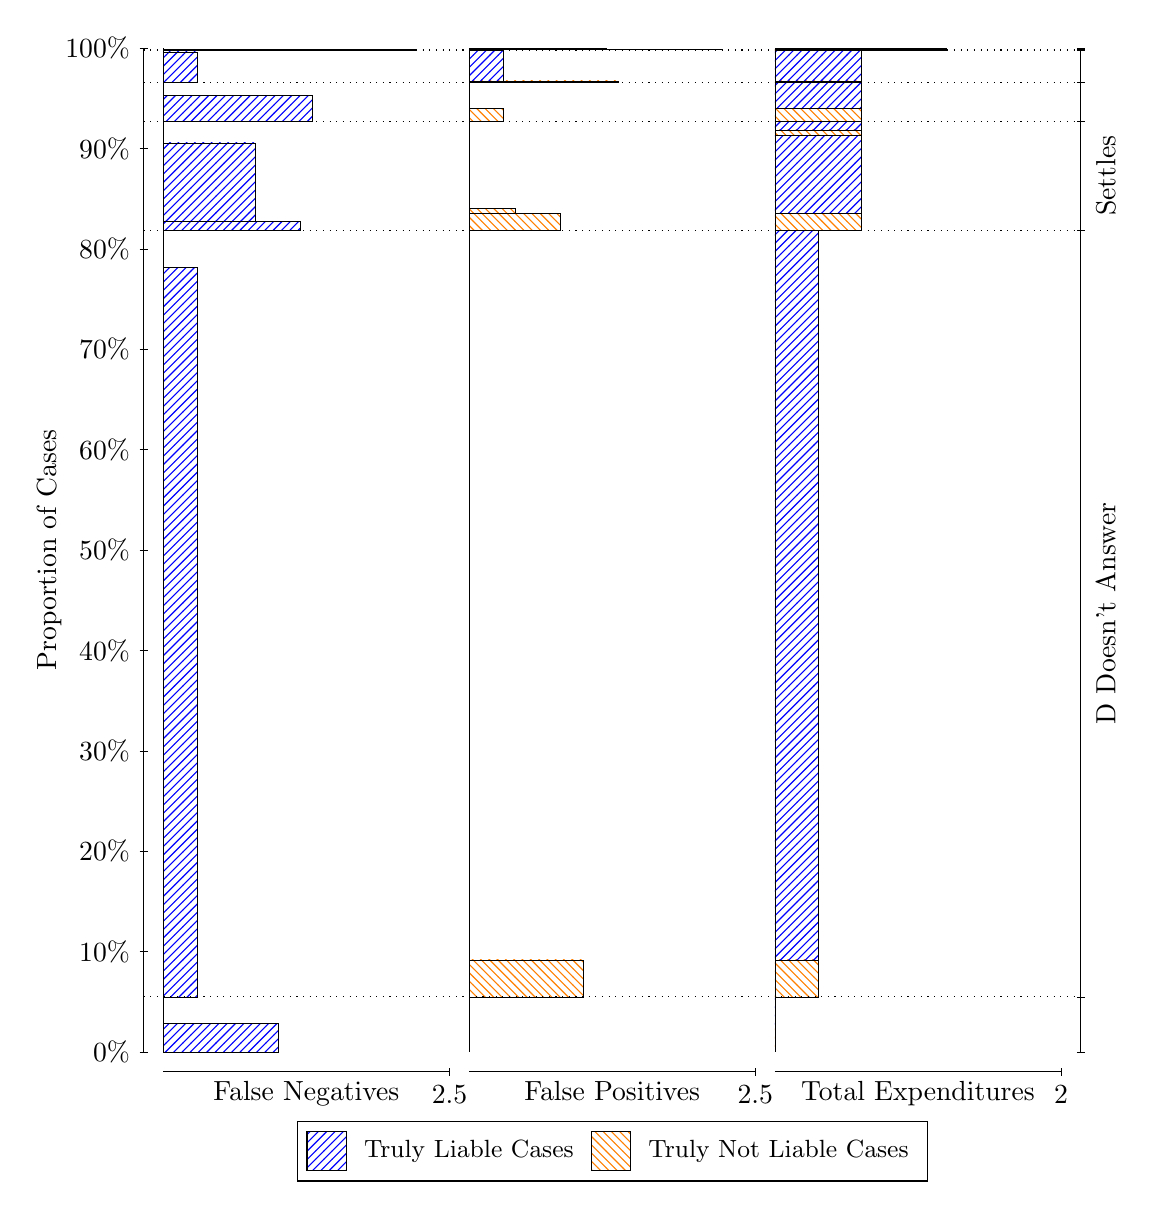
\begin{tikzpicture}
\draw[black, very thin] (1.5,1.75) -- (1.5,14.5);
\node[rotate=90, text=black, anchor=center] at (0.3, 8.125) {Proportion of Cases};
\draw[black, very thin] (1.45,1.75) -- (1.55,1.75);
\node[text=black, anchor=east] at (1.45, 1.75) {0\%};
\draw[black, very thin] (1.45,3.025) -- (1.55,3.025);
\node[text=black, anchor=east] at (1.45, 3.025) {10\%};
\draw[black, very thin] (1.45,4.3) -- (1.55,4.3);
\node[text=black, anchor=east] at (1.45, 4.3) {20\%};
\draw[black, very thin] (1.45,5.575) -- (1.55,5.575);
\node[text=black, anchor=east] at (1.45, 5.575) {30\%};
\draw[black, very thin] (1.45,6.85) -- (1.55,6.85);
\node[text=black, anchor=east] at (1.45, 6.85) {40\%};
\draw[black, very thin] (1.45,8.125) -- (1.55,8.125);
\node[text=black, anchor=east] at (1.45, 8.125) {50\%};
\draw[black, very thin] (1.45,9.4) -- (1.55,9.4);
\node[text=black, anchor=east] at (1.45, 9.4) {60\%};
\draw[black, very thin] (1.45,10.675) -- (1.55,10.675);
\node[text=black, anchor=east] at (1.45, 10.675) {70\%};
\draw[black, very thin] (1.45,11.95) -- (1.55,11.95);
\node[text=black, anchor=east] at (1.45, 11.95) {80\%};
\draw[black, very thin] (1.45,13.225) -- (1.55,13.225);
\node[text=black, anchor=east] at (1.45, 13.225) {90\%};
\draw[black, very thin] (1.45,14.5) -- (1.55,14.5);
\node[text=black, anchor=east] at (1.45, 14.5) {100\%};

\draw[black, very thin] (13.4,1.75) -- (13.4,14.5);
\draw[black, very thin] (13.35,1.75) -- (13.45,1.75);
\node[anchor=west] at (13.35, 1.75) {};
\draw[black, very thin] (13.35,2.449) -- (13.45,2.449);
\node[anchor=west] at (13.35, 2.449) {};
\draw[black, very thin] (13.35,12.186) -- (13.45,12.186);
\node[anchor=west] at (13.35, 12.186) {};
\draw[black, very thin] (13.35,13.571) -- (13.45,13.571);
\node[anchor=west] at (13.35, 13.571) {};
\draw[black, very thin] (13.35,14.064) -- (13.45,14.064);
\node[anchor=west] at (13.35, 14.064) {};
\draw[black, very thin] (13.35,14.471) -- (13.45,14.471);
\node[anchor=west] at (13.35, 14.471) {};
\draw[black, very thin] (13.35,14.482) -- (13.45,14.482);
\node[anchor=west] at (13.35, 14.482) {};
\draw[black, very thin] (13.35,14.5) -- (13.45,14.5);
\node[anchor=west] at (13.35, 14.5) {};

\draw[black, very thin, pattern color=blue, pattern=north east lines] (1.75,1.75) rectangle (3.2033,2.1094);
\draw[black, very thin, pattern color=orange, pattern=north west lines] (1.75,2.1094) rectangle (1.75,2.449);
\draw[black, very thin, pattern color=blue, pattern=north east lines] (1.75,2.449) rectangle (2.186,11.716);
\draw[black, very thin, pattern color=orange, pattern=north west lines] (1.75,11.716) rectangle (1.75,12.186);
\draw[black, very thin, pattern color=blue, pattern=north east lines] (1.75,12.186) rectangle (3.494,12.299);
\draw[black, very thin, pattern color=blue, pattern=north east lines] (1.75,12.299) rectangle (2.9127,13.294);
\draw[black, very thin, pattern color=orange, pattern=north west lines] (1.75,13.294) rectangle (1.75,13.571);
\draw[black, very thin, pattern color=blue, pattern=north east lines] (1.75,13.571) rectangle (3.6393,13.9);
\draw[black, very thin, pattern color=orange, pattern=north west lines] (1.75,13.9) rectangle (1.75,14.064);
\draw[black, very thin, pattern color=blue, pattern=north east lines] (1.75,14.064) rectangle (2.186,14.451);
\draw[black, very thin, pattern color=orange, pattern=north west lines] (1.75,14.451) rectangle (1.75,14.471);
\draw[black, very thin, pattern color=blue, pattern=north east lines] (1.75,14.471) rectangle (4.9473,14.48);
\draw[black, very thin, pattern color=orange, pattern=north west lines] (1.75,14.48) rectangle (1.75,14.482);
\draw[black, very thin, pattern color=orange, pattern=north west lines] (1.75,14.482) rectangle (1.75,14.483);
\draw[black, very thin, pattern color=blue, pattern=north east lines] (1.75,14.483) rectangle (1.75,14.5);
\draw[black, very thin, pattern color=orange, pattern=north west lines] (5.6333,1.75) rectangle (5.6333,2.0896);
\draw[black, very thin, pattern color=blue, pattern=north east lines] (5.6333,2.0896) rectangle (5.6333,2.449);
\draw[black, very thin, pattern color=orange, pattern=north west lines] (5.6333,2.449) rectangle (7.0867,2.9196);
\draw[black, very thin, pattern color=blue, pattern=north east lines] (5.6333,2.9196) rectangle (5.6333,12.186);
\draw[black, very thin, pattern color=orange, pattern=north west lines] (5.6333,12.186) rectangle (6.796,12.397);
\draw[black, very thin, pattern color=orange, pattern=north west lines] (5.6333,12.397) rectangle (6.2147,12.464);
\draw[black, very thin, pattern color=blue, pattern=north east lines] (5.6333,12.464) rectangle (5.6333,13.571);
\draw[black, very thin, pattern color=orange, pattern=north west lines] (5.6333,13.571) rectangle (6.0693,13.735);
\draw[black, very thin, pattern color=blue, pattern=north east lines] (5.6333,13.735) rectangle (5.6333,14.064);
\draw[black, very thin, pattern color=orange, pattern=north west lines] (5.6333,14.064) rectangle (7.5227,14.083);
\draw[black, very thin, pattern color=blue, pattern=north east lines] (5.6333,14.083) rectangle (6.0693,14.471);
\draw[black, very thin, pattern color=orange, pattern=north west lines] (5.6333,14.471) rectangle (5.6333,14.473);
\draw[black, very thin, pattern color=blue, pattern=north east lines] (5.6333,14.473) rectangle (5.6333,14.482);
\draw[black, very thin, pattern color=orange, pattern=north west lines] (5.6333,14.482) rectangle (8.8307,14.483);
\draw[black, very thin, pattern color=blue, pattern=north east lines] (5.6333,14.483) rectangle (7.3773,14.5);
\draw[black, very thin, pattern color=orange, pattern=north west lines] (9.5167,1.75) rectangle (9.5167,2.0896);
\draw[black, very thin, pattern color=blue, pattern=north east lines] (9.5167,2.0896) rectangle (9.5167,2.449);
\draw[black, very thin, pattern color=orange, pattern=north west lines] (9.5167,2.449) rectangle (10.062,2.9196);
\draw[black, very thin, pattern color=blue, pattern=north east lines] (9.5167,2.9196) rectangle (10.062,12.186);
\draw[black, very thin, pattern color=orange, pattern=north west lines] (9.5167,12.186) rectangle (10.607,12.397);
\draw[black, very thin, pattern color=blue, pattern=north east lines] (9.5167,12.397) rectangle (10.607,13.392);
\draw[black, very thin, pattern color=orange, pattern=north west lines] (9.5167,13.392) rectangle (10.607,13.459);
\draw[black, very thin, pattern color=blue, pattern=north east lines] (9.5167,13.459) rectangle (10.607,13.571);
\draw[black, very thin, pattern color=orange, pattern=north west lines] (9.5167,13.571) rectangle (10.607,13.735);
\draw[black, very thin, pattern color=blue, pattern=north east lines] (9.5167,13.735) rectangle (10.607,14.064);
\draw[black, very thin, pattern color=orange, pattern=north west lines] (9.5167,14.064) rectangle (10.607,14.083);
\draw[black, very thin, pattern color=blue, pattern=north east lines] (9.5167,14.083) rectangle (10.607,14.471);
\draw[black, very thin, pattern color=orange, pattern=north west lines] (9.5167,14.471) rectangle (11.697,14.473);
\draw[black, very thin, pattern color=blue, pattern=north east lines] (9.5167,14.473) rectangle (11.697,14.482);
\draw[black, very thin, pattern color=orange, pattern=north west lines] (9.5167,14.482) rectangle (11.697,14.483);
\draw[black, very thin, pattern color=blue, pattern=north east lines] (9.5167,14.483) rectangle (11.697,14.5);
\draw[black, dotted] (1.5,2.449) -- (13.4,2.449);
\draw[black, dotted] (1.5,12.186) -- (13.4,12.186);
\draw[black, dotted] (1.5,13.571) -- (13.4,13.571);
\draw[black, dotted] (1.5,14.064) -- (13.4,14.064);
\draw[black, dotted] (1.5,14.471) -- (13.4,14.471);
\draw[black, dotted] (1.5,14.482) -- (13.4,14.482);
\draw[black, very thin] (1.75,1.5) -- (5.3833,1.5);
\node[text=black, anchor=north] at (3.5667, 1.5) {False Negatives};
\draw[black, very thin] (5.3833,1.45) -- (5.3833,1.55);
\node[text=black, anchor=north] at (5.3833, 1.45) {2.5};

\draw[black, very thin] (5.6333,1.5) -- (9.2667,1.5);
\node[text=black, anchor=north] at (7.45, 1.5) {False Positives};
\draw[black, very thin] (9.2667,1.45) -- (9.2667,1.55);
\node[text=black, anchor=north] at (9.2667, 1.45) {2.5};

\draw[black, very thin] (9.5167,1.5) -- (13.15,1.5);
\node[text=black, anchor=north] at (11.333, 1.5) {Total Expenditures};
\draw[black, very thin] (13.15,1.45) -- (13.15,1.55);
\node[text=black, anchor=north] at (13.15, 1.45) {2};


\node[text=black, centered, rotate=90] at (13.72, 7.3177) {D Doesn't Answer};
\node[text=black, centered, rotate=90] at (13.72, 12.879) {Settles};





\draw (7.449999999999999,1.5) node[draw=none] (baseCoordinate) {};
\begin{scope}[align=center]
        \matrix[scale=0.5, draw=black, below=0.5cm of baseCoordinate, nodes={draw}, column sep=0.1cm]{
            \node[rectangle, draw, minimum width=0.5cm, minimum height=0.5cm, pattern color=blue, pattern=north east lines] {}; &
            \node[draw=none, font=\small, text=black] (B) {Truly Liable Cases}; &
            \node[rectangle, draw, minimum width=0.5cm, minimum height=0.5cm, pattern color=orange, pattern=north west lines] {}; &
            \node[draw=none, font=\small, text=black] (B) {Truly Not Liable Cases}; \\
            };
\end{scope}

\end{tikzpicture}
\end{document}